
\frame{\frametitle{Was ist Invisque?}
	\begin{itemize}
		\item Prototyp zur interaktiven und anschaulichen Suche
		\item Basierend auf Schreibtisch und Karteikarten Metapher
		\item Für \glqq Leseschwache\grqq in Industrienation 
	\end{itemize}
}

\frame{\frametitle{Design Gedanken}
	%dem benutzer weniger gedanken an die bedienung verschwenden lassen
	\begin{itemize}
		\item kleine Informationsstücke
		\item aufgeräumte Darstellung (\glqq page clutter\grqq)
		\item Freiraum und Farbe
		\item Animationen
		\item Verschachtelung verringern
	\end{itemize}
}

\frame{\frametitle{Evaluation}
\begin{columns}
	\column{0.5\textwidth}
	\begin{itemize}
		\item 24 Testpersonen
		\item zwölf Frauen und zwölf Männer
		\item zwölf \glqq Lesestarke\grqq und zwölf \glqq Leseschwache\grqq
		\item zwischen 35 und 50 Jahre alt
		\item zwischen fünf und zehn Stunden Computer- und Internetnutzung in der Woche
		%bild der Ergebnisse
	\end{itemize}
	
	\column{0.5\textwidth}
	\begin{figure}
		\centering
		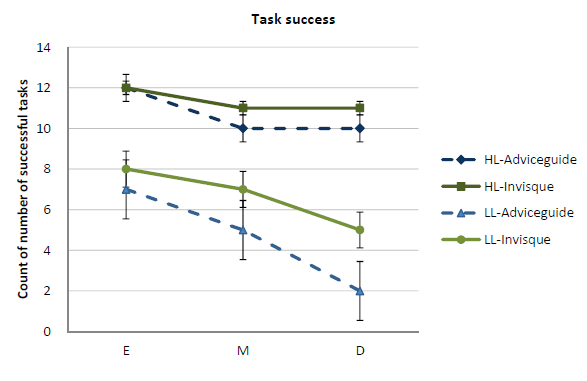
\includegraphics[width=\textwidth]{Slides/Anwendungen/Daten/pics/success.png}
	\end{figure}
\end{columns}
}

\frame{\frametitle{Demo}

}
